\section{引言}
\label{sec:introduction}

住宅平面图的自动化生成是计算机辅助建筑设计的核心问题之一。
理想的系统应当允许设计师以自然语言表达设计意图
（如"客厅居中，两侧各有一间卧室，厨房通过走廊与卫生间相连"），
并自动生成与描述一致、拓扑合理的矢量平面图。

早期工作主要依赖图约束或气泡图（bubble diagram）作为生成条件~\cite{nauata2020housegan,shabani2023housediffusion}。
这类方法虽能输出几何上连贯的平面图，
但气泡图本身仍需由设计师手工绘制，并未从根本上解决"从语言到图纸"的端到端生成问题。
Architext~\cite{galanos2023architext} 率先将大语言模型引入平面图生成，
但其文本描述由规则模板自动生成，语言单一，与真实设计需求存在较大差距。
ChatHouseDiffusion~\cite{qin2025chathousediffusion} 进一步引入 prompt 引导并支持局部编辑，
但侧重于像素级图像生成，尚未面向矢量图结构的显式拓扑建模。

本文提出 \textbf{PlanDiffusion}，一种以\textbf{图结构为中间表示}的文本驱动平面图生成框架，
整体流程如图~\ref{fig:overview} 所示。
核心思路是将生成任务分解为三个串联阶段：
（1）\textbf{图拓扑生成}：以 LLaMA 自回归模型将文本描述转化为平面图的拓扑图结构，
包括节点数量与邻接关系；
（2）\textbf{节点坐标扩散}：以图结构和文本为双重条件，
通过去噪扩散概率模型（DDPM）生成每个顶点的二维坐标；
（3）\textbf{节点类型预测}：以生成坐标、图结构和文本为条件，
通过独立分类器预测每个节点的房间组合类型。
显式的图结构中间表示使拓扑约束在扩散过程中始终可控，
同时为坐标生成提供了强结构先验；
类型预测与坐标扩散完全解耦，在干净坐标上以纯监督方式训练。

为支撑上述框架的训练，我们在 Architext\_v1~\cite{galanos2023architext} 基础上构建了
\textbf{PlanText-150K}，一个包含 \textbf{149,950} 条样本的大规模平面图-文本数据集。
与原始数据集的模板式描述不同，
我们调用 MiMo-V2.5 视觉语言模型对每张平面图生成自然语言描述，
并经人工抽查校正，显著提升了文本标注的多样性与自然度。

本文的主要贡献如下：
\begin{itemize}
    \item 提出以图结构为中间表示的三阶段文本驱动平面图生成框架，
    在保证拓扑合法性的同时实现端到端的语言条件生成；
    \item 设计了"BFS 生成树 + 补边"的图序列化格式，
    使任意连通图均可被自回归语言模型高效建模；
    \item 构建了 PlanText-150K 数据集，
    通过 MiMo-V2.5 VLM 自动标注并经人工抽查校正提供高质量自然语言描述，
    是目前规模最大的带文本标注的住宅平面图数据集之一；
    \item 设计了三流注意力去噪网络（NodeDiffusionTransformer），
    并联邻接局部注意力（AdjAttn）、面结构注意力（RoomAttn）与全局注意力（GlobalAttn），
    分别捕捉节点的局部边约束、房间面约束与全局布局信息，
    在纯文本条件下高精度恢复节点坐标；
    并在此基础上扩展四流轮廓条件变体（PlanDiffusion-bnd），
    以外轮廓节点固定 + BndAttn 提供等价于 ChatHouseDiffusion 轮廓输入的几何约束，
    实现公平定量对比。
\end{itemize}

\begin{figure}[t]
    \centering
    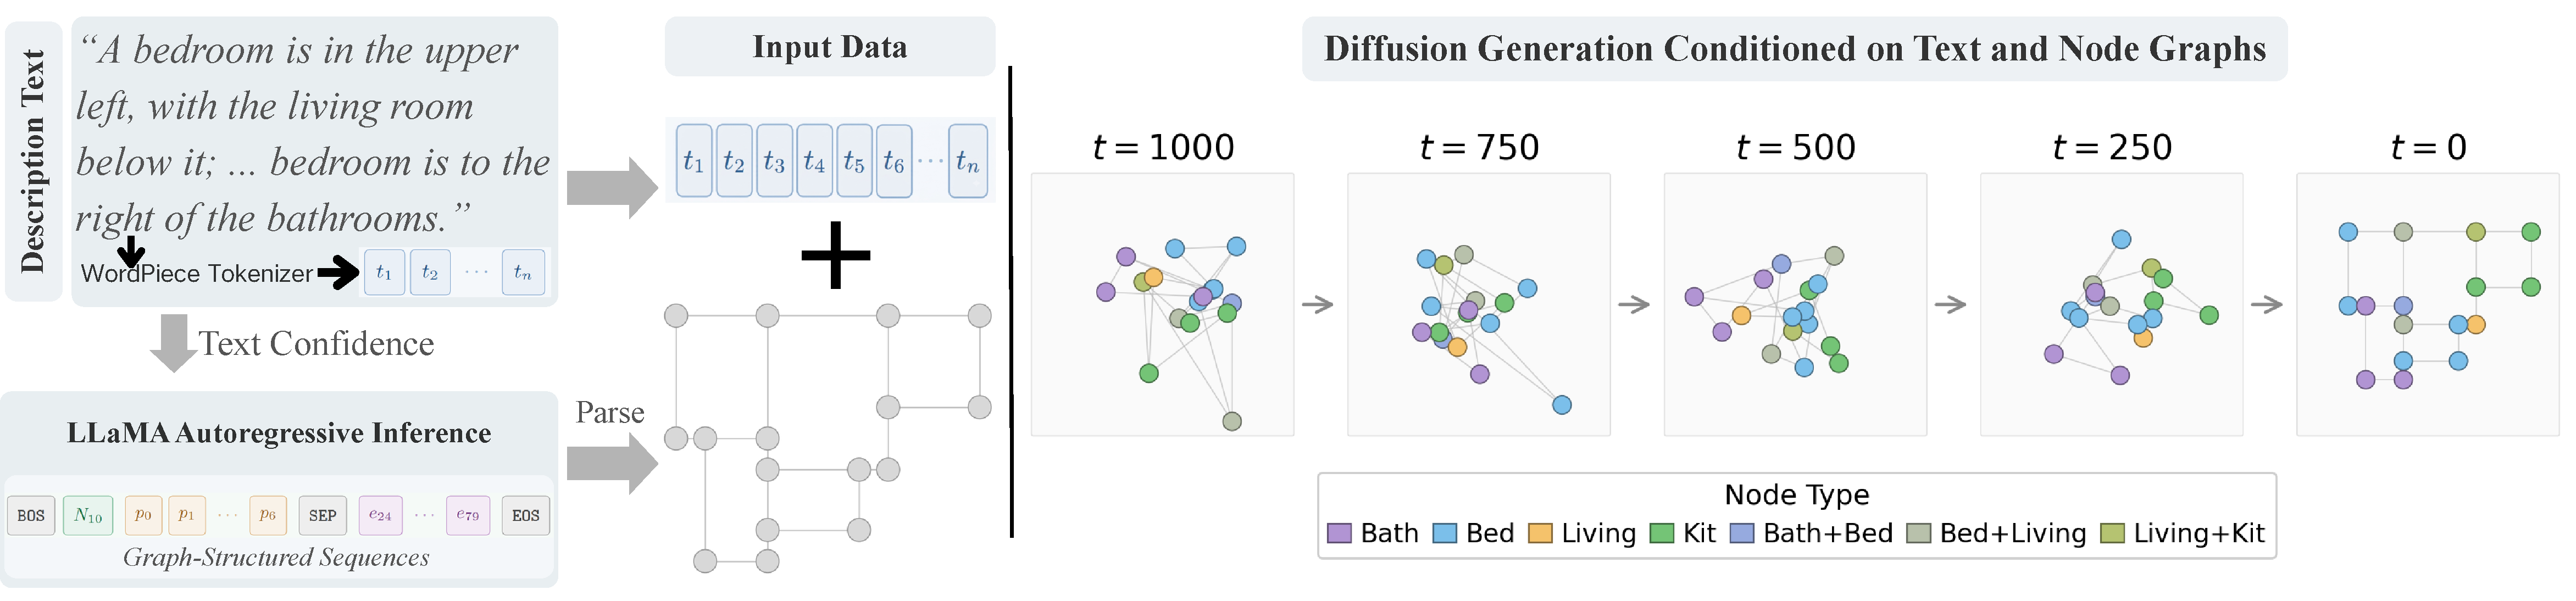
\includegraphics[width=\textwidth]{figures/total_process.pdf}
    \caption{
        PlanDiffusion 整体流程。
        左：图拓扑生成阶段以文本描述为条件，通过 LLaMA 自回归推理生成图结构序列，
        解析得到顶点图；
        右：完整三阶段生成过程——$\theta_2$ 以顶点图和文本为条件，
        通过 DDPM 逆扩散从高斯噪声（$t=1000$）逐步恢复节点坐标（$t=0$）；
        随后 $\theta_3$ 对节点进行类型预测，最终通过半边遍历与投票渲染输出彩色平面图。
    }
    \label{fig:overview}
\end{figure}
